\chapter{Webapp}
\label{ch:Webapp}

\author{Nico Leidenfrost}

After the conclusion that an Android application would not satisfy all the requirements of GRAMOC, the decision to build a Web application was made. A so called ``Webapp'' is an application that runs inside a web browser (e.g. Google Chrome) and is usually provided by a web server. After a user connects to the web server, the user will get application files and data, this enables the ability of a Webapp to be platform independent.

\section{Framework}
To develop a modern Webapp a developer should choose a framework to build this web application. A software framework can be identified as a software library, it provides basic functionality like rendering content or routing between views in the case of a web framework. The biggest advantage of a web framework is that the developer does not need to reinvent the wheel, because a framework already provides the basic functionalities, also most of the frameworks out there are open source, which means thousands of people can contribute to the project and also find and fix bugs as well as issues. Therefore the user gains a solid code base which is efficient, secure and in most cases well documented.

\subsection{Vue.js}
In the case of GRAMOC a framework called ``Vue.js'' was chosen because of the performance compared to other big frameworks and the ``simplicity and ease of use'', as stated in a blog post written by the Frontend DC Lead of GitLab \cite{Vue} \cite{WhyVue} \cite{GitLab}. The performance was measured with the benchmark application from Stefan Krause, the results are partitioned in keyed and non keyed implementations \cite{FrameworkBenchmark}. The distinct each other in the way the data items are bind to the DOM (Document Object Model) node. The keyed implementation assigns a key to each node and the non keyed just updates the data inside of that particular node, therefore the non keyed implementation can achieve a higher performance since costly DOM operations like constantly removing and adding nodes can be avoided.

Following table shows the average time in milliseconds each operation takes:

\begin{table}[H]
    \centering
    \begin{tabular}{| C{2.2cm} | C{1.5cm} | C{1.5cm} | C{1.5cm} | C{1.5cm} | C{1.5cm} | C{1.5cm} |}
    \hline
    \textbf{Name} & \textbf{Vue v2.4.4 non-keyed} & \textbf{Angular v4.4.3 non-keyed} & \textbf{React v15.5.4 non-keyed} & \textbf{Vue v2.4.4 keyed} & \textbf{Angular v4.4.3 keyed} & \textbf{React v15.5.4 keyed} \\ \hline
    \textbf{create 1000 rows after the page loaded} & 176.1 & 189.4 & 192.0 & 178.2 & 208.8 & 189.7 \\ \hline
    \textbf{update all 1000 rows of the table} & 63.6 & 61.0 & 75.7 & 172.6 & 194.0 & 185.7 \\ \hline
    \textbf{update every 10th row for a table with 10000 rows} & 131.6 & 79.9 & 106.4 & 136.8 & 77.4 & 106.1 \\ \hline
    \textbf{highlight a row in response to a click on the row} & 12.0 & 9.9 & 8.2 & 10.1 & 5.9 & 9.9 \\ \hline
    \textbf{swap two rows on a table with 1000 rows} & 17.8 & 13.9 & 14.5 & 20.9 & 17.8 & 17.4 \\ \hline
    \textbf{remove a row} & 41.0 & 36.8 & 47.7 & 50.9 & 46.8 & 48.3 \\ \hline
    \textbf{create 10000 rows} & 1622.0 & 1713.4 & 1768.1 & 1610.7 & 1665.3 & 1767.0 \\ \hline
    \textbf{add 1000 rows to a table with 10000 rows} & 329.2 & 283.2 & 294.8 & 339.0 & 270.6 & 298.0 \\ \hline
    \textbf{clear a table filled with 10000 rows} & 260.4 & 375.5 & 393.1 & 251.3 & 350.4 & 362.4 \\ \hline
    \textbf{time for loading, parsing and starting up} & 48.7 & 92.6 & 58.6 & 48.2 & 92.2 & 60.4 \\ \hline
    \textbf{slowdown geometric mean} & 1.11 & 1.14 & 1.19 & 1.28 & 1.31 & 1.30 \\
    \hline
    \end{tabular}
    \caption{The measured time cost of given operations by each framework (slowdown = duration / fastest)}
    \label{tab:framework_perf_dur}
\end{table}

Following table shows the average memory allocation in Megabyte:

\begin{table}[H]
    \centering
    \begin{tabular}{| C{2.2cm} | C{1.5cm} | C{1.5cm} | C{1.5cm} | C{1.5cm} | C{1.5cm} | C{1.5cm} |}
    \hline
    \textbf{Name} & \textbf{Vue v2.4.4 non-keyed} & \textbf{Angular v4.4.3 non-keyed} & \textbf{React v15.5.4 non-keyed} & \textbf{Vue v2.4.4 keyed} & \textbf{Angular v4.4.3 keyed} & \textbf{React v15.5.4 keyed} \\ \hline
    \textbf{Memory usage after page load} & 3.2 & 7.3 & 3.9 & 3.2 & 7.2 & 4.0 \\ \hline
    \textbf{Memory usage after adding 1000 rows} & 7.0 & 14.9 & 8.8 & 7.0 & 12.9 & 8.9 \\
    \hline
    \end{tabular}
    \caption{The measured memory used by each framework}
    \label{tab:framework_perf_mem}
\end{table}

In order to use Vue.js it is recommended by the developers to use ``webpack''  as module bundler and ``Babel'' as JavaScript compiler \cite{webpack} \cite{Babel}.

\subsubsection{webpack}
webpack is a module bundler for modern JavaScript applications, that builds a dependency graph which includes every module needed to execute the application. It packages all the needed modules into one or more bundles which can be used as static asserts.

\subsubsection{Babel}
Babel is a JavaScript compiler that gives the developer the ability to write code in the latest version of JavaScript and if the targeted environment does not support these version, Babel compiles the code to a supported prior version.

\section{Web Server}
To make a web application accessible to a user, there needs to be a web server which serves the files to the web browser of the user. In the case of GRAMOC ``Node.js'' with its built-in module HTTP was chosen to be used as a web server \cite{Node}.

\subsection{Node.js}
Node.js is a asynchronous event driven JavaScript runtime, designed to build network applications \cite{Node}. To use Node as a web server a developer must use the built-in module HTTP, which allows to transfer data over the HTTP protocol, but there is also a module that can handle IPC connections. The main function of the Node server is to receive data from the Filtering and Preprocessing Layer (FAPS) and forward it to the web application via web sockets implemented through the ``socket.io'' library \cite{socketio}. The Webapp itself is served by ``Express'' \cite{express}.

\subsection{socket.io}
socket.io is a JavsScript client library to be used in combination with Node.js. This library was chosen because it aims to make real-time applications possible in every browser. Since GRAMOC was built with the intent of delivering sensor data in real-time to the user, socket.io helped a lot in the step of implementing real-time communication.

\subsection{Express}
Express is a minimal and flexible web application framework to be used with Node.js. It is build on top of the HTTP module thats included in the standard library from Node.js and its main focus is to handle the routing tasks of the HTTP server running. So it is not a web server itself, but a layer on top of it to provide some extra features.

\section{Plotly}
To visualize the data received from the sensor a graphing library called ``Plotly'', more specific the open source JavaScript library ``plotly.js'' \cite{Plotly} \cite{PlotlyJS}. Plotly is build on top of state of the art JavaScript libraries like ``d3.js''  and ``stackgl'' \cite{d3} \cite{stackgl}. The library offers a broad variety of two and three dimensional charts in the categories statistical, financial, scientific and more. Plotly was chosen because of the capability to easily create custom, dynamic and real time charts.

\section{Workflow}

As shown in figure \ref{fig:webserver-program-flow} the server asynchronously tries to connect with the IPC socket and starts listening for incoming connections on a specified port. The server keeps retrying to connect to the IPC socket until a connection is established because without this connection no data can be forwarded to the web application. If a client connects on the before specified port the connection will be immediately upgraded to a socket connection and the web application will be served to the user. When the Webapp launches it will display the Home page, then the user can navigate to the 2D, the 3D or the About page, through the navigation bar at the top. If the About page was selected the user simply gets a static about page. If the user navigates to the 2D page, three line charts will be initialized and the client emits a message to the server to start receive the sensor data. This data will be used to update the charts accordingly.
\todo{explain what data the 2d charts display}
\todo{explain the extra features like saving, stopping...}
\todo{write about the 3d page}

\begin{figure}[H]
    \centering
    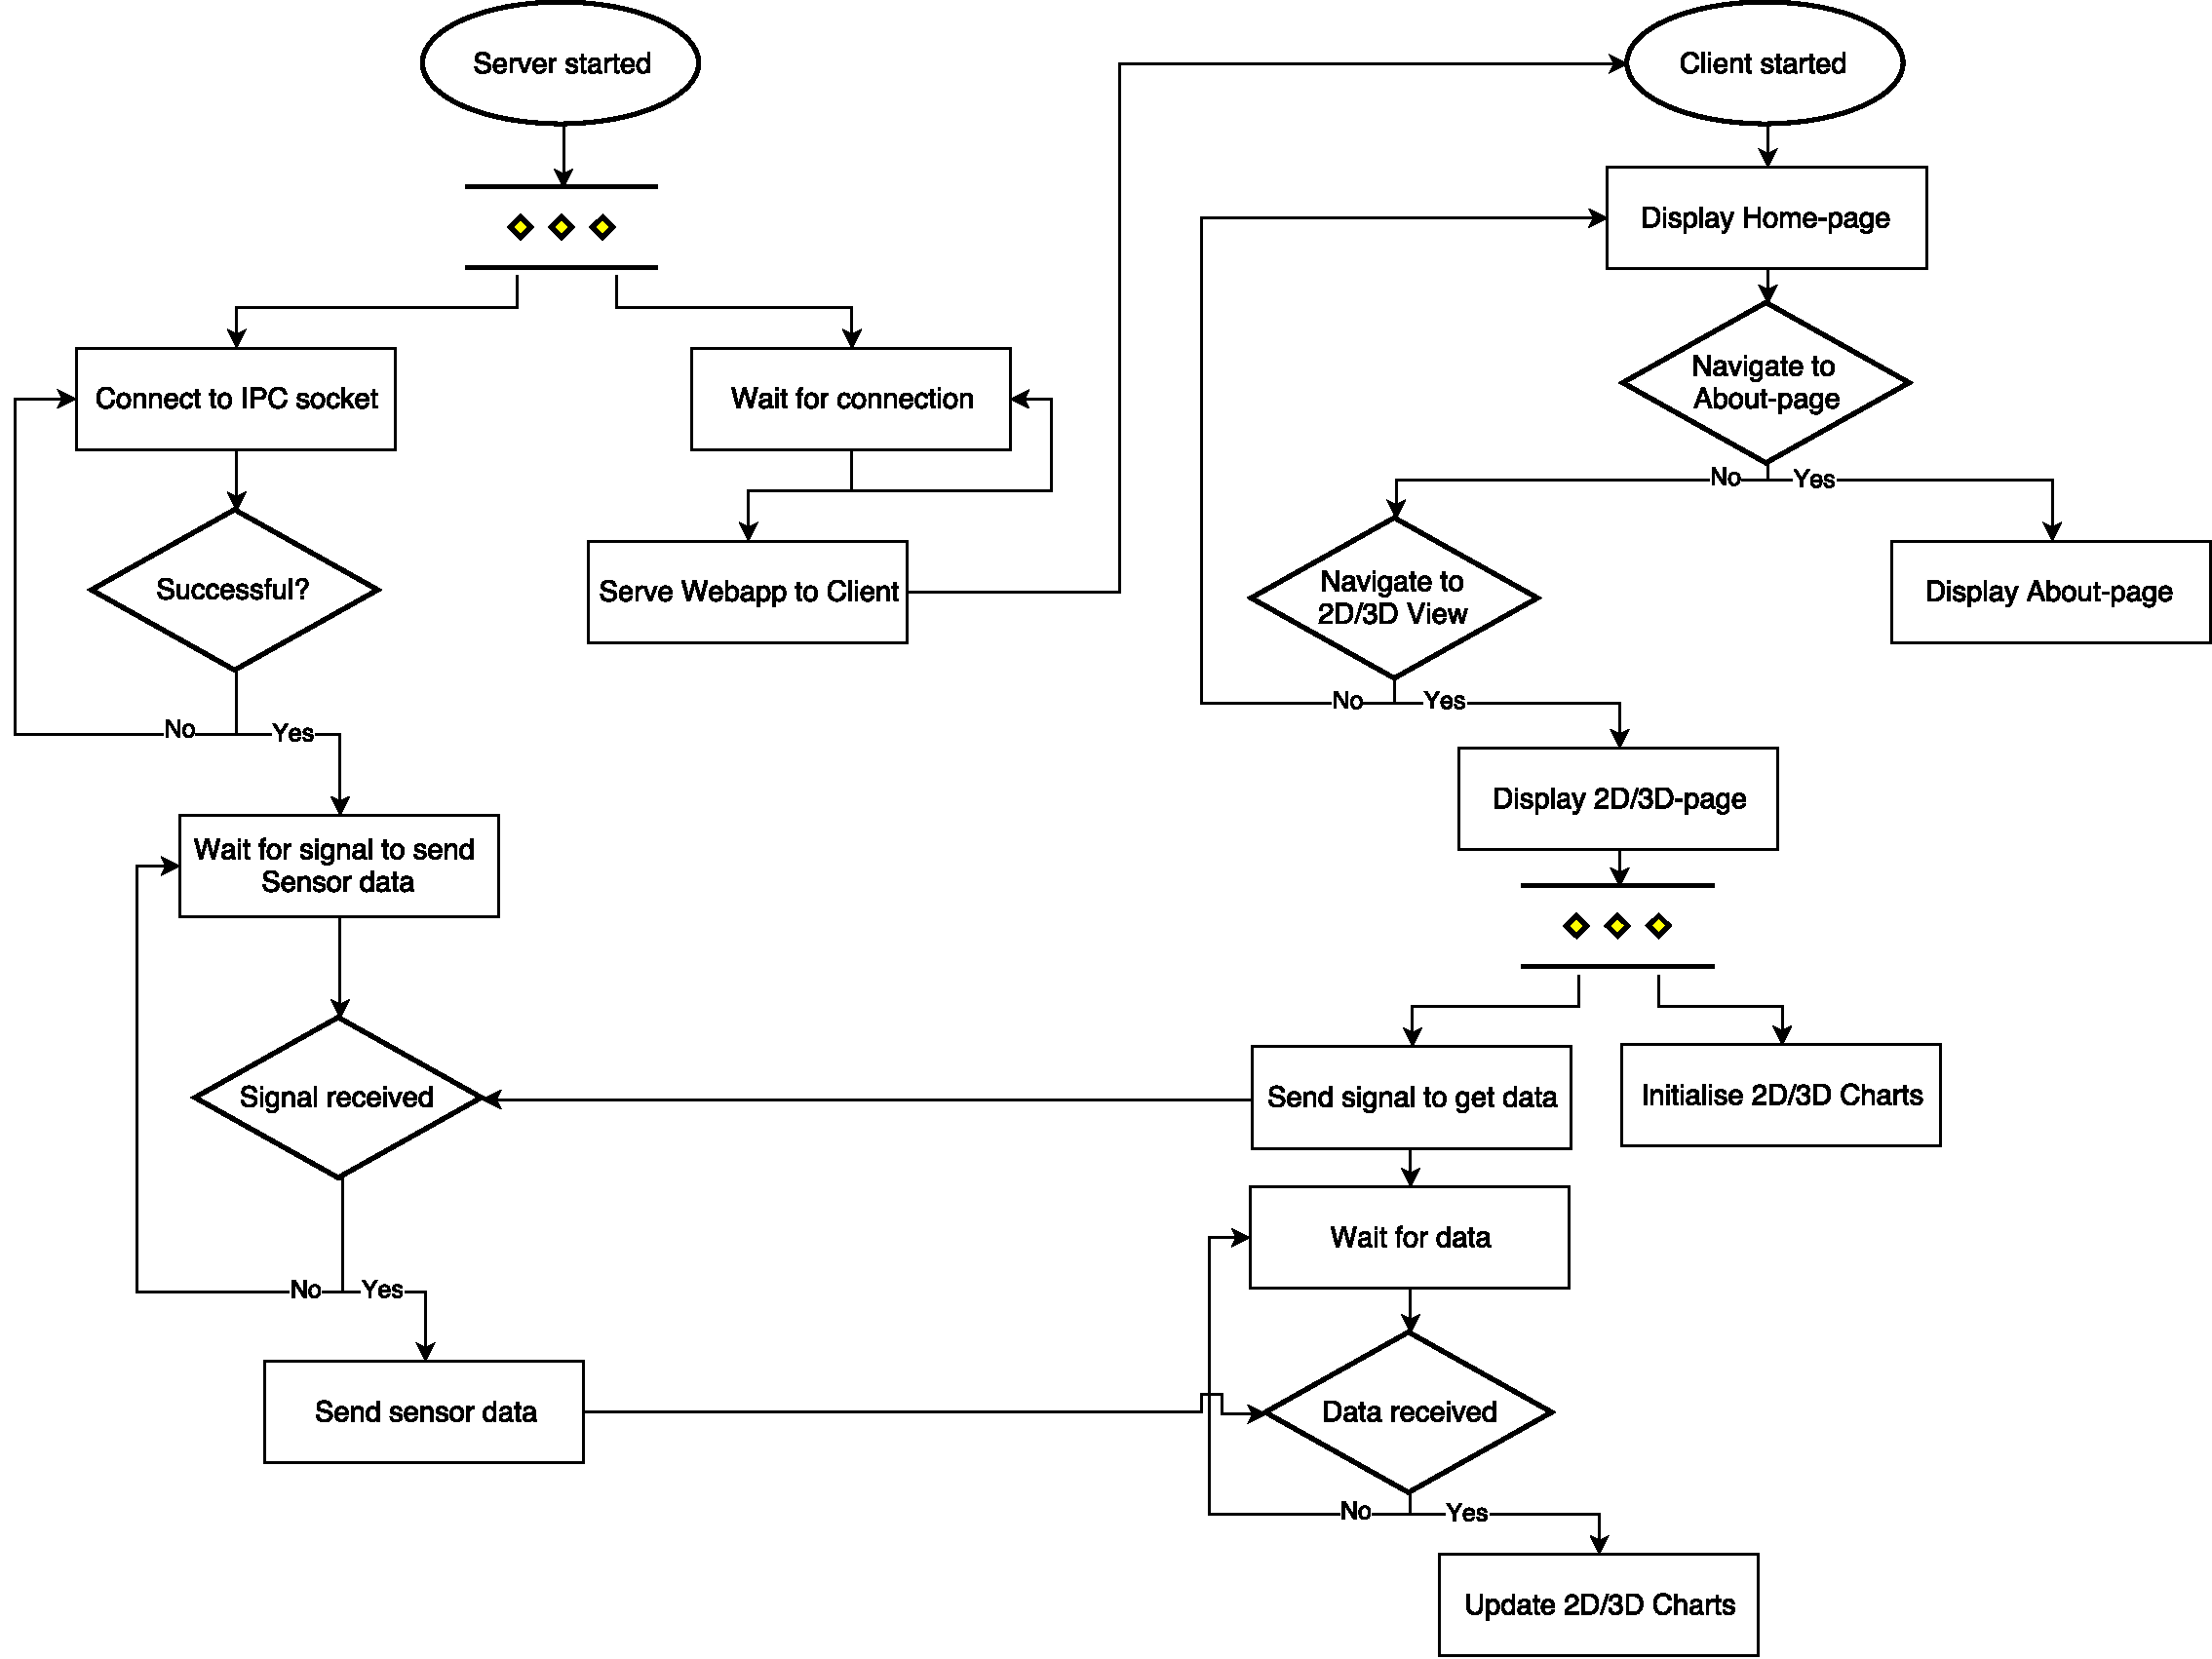
\includegraphics[width=15cm,keepaspectratio]{webserver-task}
    \caption{Flowchart of web server and client program showing the procedure}
    \label{fig:webserver-program-flow}
\end{figure}
